% Provenance (never printed): see sources/outline_sources.md (Year 2: the solar nebula
% and the condensation sequence; planetesimals and embryos; chondrites, achondrites and
% irons; the age of the Solar System; differentiation of planets). Curves from
% figdata/bachelor-2/nebula.py, condensation.py, al26.py, meteorites.py; exercise and
% problem values in the Book 4 scratch calculator calc/ch02.py.
\chapter{Pembentukan Planet dan Meteorit}\label{ch:b2:planet-formation-meteorites}

Setiap tahun sekitar lima belas ribu ton debu dari antariksa memasuki atmosfer Bumi;
sebagian besar terbakar habis atau mengendap sebagai sferul mikroskopis, dan sesekali
sebongkah batu seukuran kepalan tangan jatuh disertai bola api dan dentuman sonik.
Sebagian besar batu ini adalah pecahan asteroid, dan banyak di antaranya hampir tidak
berubah sejak terbentuk. Belahlah sebongkah dan poleslah, maka tampak butir-butir
berukuran milimeter dari batuan yang dahulu cair, butiran putih tak beraturan dari mineral
kalsium dan aluminium, serpihan logam, semuanya terikat dalam semen gelap berbutir halus.
Butiran putih itu adalah zat padat tertua di Tata Surya: isotop timbal menentukan umurnya
4567 juta tahun. Jam kedua, yaitu peluruhan isotop radioaktif aluminium yang sudah lama
lenyap, menentukan umur komponen-komponen lain relatif terhadap butiran itu dengan ketelitian
sepersekian juta tahun. Bab ini mengikuti cakram dari bab sebelumnya saat cakram itu
berubah menjadi planet-planet: zat padat apa yang mengembun dari gas yang mendingin, dan di
mana; bagaimana debu tumbuh menjadi benda berukuran kilometer lalu menjadi planet; apa
\omterm{def:b2:planet-formation-meteorites:fall-find}{meteorit} itu, dan bagaimana \omterm{def:b2:planet-formation-meteorites:fall-find}{meteorit} menentukan umur peristiwa-peristiwa ini; dan mengapa
sebagian benda pertama melebur dan menumbuhkan inti besi sementara yang lain tetap seperti
saat terbentuk.
% ledger: rojas21:flux, lugaro:cai, gail:meteorites

\begin{recall}
Bintang-bintang muda dikelilingi \omterm{def:b2:ism-star-formation:disc}{cakram protoplanet}, yang lenyap dalam beberapa juta
tahun; sebutir debu dalam cahaya bintang pada jarak $r$ dari bintang berluminositas
$L$ menetap pada $T = \bigl(L/(16\pi\sigma r^2)\bigr)^{1/4}$
(\cref{ch:b2:ism-star-formation}). Asteroid adalah benda kecil berbatu atau berlogam
di Tata Surya, yang sebagian besar mengorbit di antara Mars dan Jupiter (volume
Tahun 1). Inti radioaktif meluruh dengan peluang $\lambda$ per satuan
waktu: $N = N_0 e^{-\lambda t}$; waktu paruhnya $\ln 2/\lambda$, dan umur
rata-ratanya $\tau = 1/\lambda$ (fisika). Dalam sistem tertutup, sampel-sampel kogenetik
dengan perbandingan induk terhadap anak yang berbeda terletak pada satu garis lurus, isokron,
yang kemiringannya memberikan umur dan titik potongnya adalah perbandingan awal (volume Tahun 1).
Memanaskan massa $m$ berkapasitas kalor jenis $c$ sebesar $\Delta T$ memerlukan energi
$mc\,\Delta T$ (fisika).
\end{recall}

\section{Nebula surya}

\begin{definition}[Nebula surya]\label{def:b2:planet-formation-meteorites:nebula}
Yang disebut \emph{nebula surya}\index{nebula surya} adalah \omterm{def:b2:ism-star-formation:disc}{cakram protoplanet} berisi gas
dan debu yang mengelilingi Matahari muda dan menjadi asal terbentuknya planet-planet,
satelit-satelitnya, asteroid, dan komet.
\end{definition}

Berapa banyak materi yang dimuatnya? Batas bawahnya berasal dari planet-planet itu sendiri.
Tambahkan pada setiap planet hidrogen dan helium secukupnya agar komposisinya sama dengan
Matahari, sebarkan hasilnya pada sebuah cincin yang berpusat pada orbitnya, maka kerapatan
permukaan, yaitu massa per satuan luas cakram, menurun terhadap jarak dari
Matahari. Rekonstruksi ini adalah \emph{nebula surya bermassa
minimum}\index{nebula surya bermassa minimum}. Dalam versi yang banyak dipakai, kerapatan
permukaan gasnya adalah
\[
  \Sigma_g = \qty{2200}{g.cm^{-2}}\left(\frac{r}{\qty{1}{au}}\right)^{-3/2},
\]
dan kerapatan permukaan zat padatnya $\Sigma_p = \qty{33}{g.cm^{-2}}\,Z_{\mathrm{rel}}\,
(r/\qty{1}{au})^{-3/2}$, dengan $Z_{\mathrm{rel}}$ adalah fraksi materi yang dapat
mengembun yang benar-benar padat: $0.33$ di tempat hanya batuan dan logam yang telah
mengembun, sekitar $0.78$ di tempat es air telah bergabung dengannya, $1$ di luar tempat
metana membeku. Angka-angka ini tidak pasti: kandungan unsur berat
Jupiter hanya diketahui dalam batas faktor empat, dan planet-planet tidak harus
terbentuk di tempat orbitnya sekarang.
% ledger: cy10:mmsn

\begin{proposition}[Massa sebuah cakram]\label{prop:b2:planet-formation-meteorites:disc-mass}
Cakram berkerapatan permukaan $\Sigma(r) = \Sigma_1 (r/r_1)^{-3/2}$ memuat, di dalam
jari-jari $R$, massa
\[
  M(R) = 4\pi\Sigma_1 r_1^2 \left(\frac{R}{r_1}\right)^{1/2}.
\]
Sebagian besar massanya terletak jauh di luar: menggandakan jari-jari menambah massa
sebesar \qty{41}{\percent}.
\end{proposition}

\begin{proof}
Sebuah cincin berjari-jari $r$ dan selebar $\mathrm dr$ memiliki luas $2\pi r\,\mathrm dr$, sehingga
\[
  M(R) = \int_0^R 2\pi r\,\Sigma_1 \left(\frac{r}{r_1}\right)^{-3/2}\mathrm dr
       = 2\pi\Sigma_1 r_1^{3/2}\int_0^R r^{-1/2}\,\mathrm dr
       = 4\pi\Sigma_1 r_1^{3/2} R^{1/2},
\]
yang merupakan rumus tadi; integralnya konvergen di $r = 0$. Menggandakan $R$
mengalikan $M$ dengan $\sqrt 2 = 1.41$.
\end{proof}

Dengan $\Sigma_1 = \qty{2.2e4}{kg.m^{-2}}$ pada $r_1 = \qty{1}{au}$, nebula bermassa minimum
memuat $0.03$ massa Matahari di dalam \qty{100}{au} (\cref{exo:b2:planet-formation-meteorites:5}). Cakram-cakram
yang teramati di sekitar bintang berumur sejuta tahun, yang ditimbang melalui pendar milimeter
debunya, memuat \numrange{0.001}{0.1} massa Matahari: nebula bermassa minimum
dengan nyaman berada di antaranya.
% ledger: cy10:mmsn

Hampir seluruh massa ini berupa gas yang tidak akan pernah mengembun. Matahari lahir
dengan fraksi massa hidrogen $X_0 = 0.711$, helium $Y_0 = 0.274$, dan
semua unsur yang lebih berat bersama-sama hanya $Z_0 = 0.0149$. Mendinginkan gas berkomposisi
ini sampai segala yang dapat membeku telah membeku hanya mengubah
\qty{1.5}{\percent} massanya menjadi zat padat: \qty{0.49}{\percent} batuan dan
logam, dan \qty{1.0}{\percent} es air, metana, dan amonia, dengan es air
saja \qty{0.57}{\percent}. Semua planet berbatu, dan inti planet-planet
raksasa, dibangun dari fraksi kecil ini.
% ledger: lodders:protosolar, lodders:condensates

Suhu cakram menentukan apa yang padat di mana. Cakram yang hanya dipanaskan oleh
bintangnya, yaitu cakram \emph{pasif}, hangat di permukaannya, tempat butiran melihat
bintang secara langsung (proposisi pada \cref{ch:b2:ism-star-formation}), dan
jauh lebih dingin di bidang tengahnya, yang hanya menerima inframerah yang dipancarkan
ulang oleh butiran-butiran permukaan itu. Untuk bintang muda bermassa satu massa Matahari,
model cakram semacam itu memberikan suhu bidang tengah
\[
  T = \qty{120}{K}\left(\frac{r}{\qty{1}{au}}\right)^{-3/7}.
\]
Akresi gas melalui cakram, yang melepaskan energi gravitasi, membuat
bidang tengah lebih panas, terutama pada awalnya dan di dekat bintang (gambar di bawah).
% ledger: cy10:passive

\begin{omfigure}
\begin{tikzpicture}
\begin{axis}[omrecord, width=0.82\linewidth, height=6.2cm, xmode=log, ymode=log,
  xmin=0.1, xmax=100, ymin=10, ymax=1000,
  xlabel={jarak dari bintang $r$ (au)}, ylabel={suhu (K)},
  tick label style={font=\scriptsize}, label style={font=\small},
  legend pos=north east, legend style={font=\scriptsize, draw=black!30}]
\addplot[thick, red!70!black] table[x=r_au, y=T_grain] {figdata/out/bachelor-2-nebula-temp.dat};
\addlegendentry{butiran dalam cahaya bintang langsung}
\addplot[thick, blue!70!black] table[x=r_au, y=T_mid] {figdata/out/bachelor-2-nebula-temp.dat};
\addlegendentry{bidang tengah cakram pasif}
\addplot[black!50, densely dashed, domain=0.1:100, samples=2] {182};
\addplot[black!50, densely dashed, domain=0.1:100, samples=2] {41};
\node[font=\scriptsize, anchor=south east] at (axis cs:95,182) {es air, \qty{182}{K}};
\node[font=\scriptsize, anchor=north west] at (axis cs:0.46,41) {es metana, \qty{41}{K}};
\draw[blue!70!black, -latex] (axis cs:0.38,25) -- (axis cs:0.38,175);
\node[font=\scriptsize, blue!70!black, anchor=north] at (axis cs:0.38,25) {\qty{0.4}{au}};
\draw[red!70!black, -latex] (axis cs:2.34,25) -- (axis cs:2.34,175);
\node[font=\scriptsize, red!70!black, anchor=north] at (axis cs:2.34,25) {\qty{2.3}{au}};
\end{axis}
\end{tikzpicture}

\par\smallskip{\small Dua suhu cakram di sekitar bintang berluminositas satu luminositas Matahari.
Merah: butiran hitam dalam cahaya bintang langsung (\cref{ch:b2:ism-star-formation}). Biru:
bidang tengah cakram pasif di sekitar bintang muda bermassa Matahari, yang terlindung dari cahaya
langsung. Es air stabil di bawah \qty{182}{K}: panah-panah menandai tempat setiap kurva
memotong garis itu. \omterm{def:b2:planet-formation-meteorites:snow-line}{Garis salju} yang sebenarnya terletak di antara batas-batas semacam itu dan
bergeser seiring evolusi cakram. Data: Chiang dan Youdin (2010); Lodders (2003).}
% ledger: cy10:passive, lodders:phases, cy10:mmsn, sun:L, const:sigma
\end{omfigure}

\section{Urutan kondensasi}

Bayangkan gas nebula, di dekat Matahari muda, cukup panas sehingga setiap
unsur berupa uap, lalu biarkan gas itu mendingin cukup lambat agar gas dan zat padat
tetap dalam kesetimbangan kimia. Ketika suhu turun, setiap unsur
bergiliran meninggalkan gas menuju zat padat, baik sebagai senyawanya sendiri maupun
terlarut dalam zat padat yang telah terbentuk.

\begin{definition}[Suhu kondensasi, urutan kondensasi]
\label{def:b2:planet-formation-meteorites:condensation}
Yang disebut \emph{suhu kondensasi}\index{suhu kondensasi} sebuah
unsur dalam gas yang mendingin dengan komposisi dan tekanan tertentu adalah suhu
saat separuh unsur itu telah beralih menjadi zat padat dalam kesetimbangan kimia
(\emph{suhu kondensasi 50 persen}; suhu saat zat padat pertamanya muncul
adalah suhu \emph{kemunculan}). Yang disebut
\emph{urutan kondensasi}\index{urutan kondensasi} adalah urutan munculnya
unsur-unsur dan senyawa padatnya ketika gas mendingin.
\end{definition}

Perhitungan untuk gas berkomposisi Matahari dilakukan pada tekanan total
$10^{-4}$ bar, yang khas untuk nebula di dekat \qty{1}{au}. Zat padat pertama adalah
oksida aluminium dan kalsium (tabel di bawah), yang terbentuk pada sekitar
\qty{1700}{K}; sebagian besar materi pembentuk batuan, yaitu silikat magnesium dan
logam besi, mengembun di dekat \qty{1350}{K}; besi sulfida menunggu hingga
\qty{704}{K}, dan es air hingga \qty{182}{K}.
% ledger: lodders:phases

\begin{table}[h]
\centering
\small
\begin{tabular}{lll}
\hline
zat padat & rumus & muncul pada (K)\\
\hline
korundum & \ce{Al2O3} & 1677\\
hibonit & \ce{CaAl12O19} & 1659\\
perovskit & \ce{CaTiO3} & 1593\\
spinel & \ce{MgAl2O4} & 1397\\
logam besi--nikel & \ce{Fe}, dengan \ce{Ni}, \ce{Co}, \ce{Cr} & 1357\\
forsterit & \ce{Mg2SiO4} & 1354\\
schreibersit & \ce{Fe3P} & 1248\\
troilit & \ce{FeS} & 704\\
magnetit & \ce{Fe3O4} & 371\\
es air & \ce{H2O} & 182\\
hidrat amonia & \ce{NH3.H2O} & 131\\
klatrat metana & \ce{CH4.7H2O} & 78\\
\hline
\end{tabular}
\caption{\omterm{def:b2:planet-formation-meteorites:condensation}{Urutan kondensasi} gas berkomposisi Tata Surya pada
$10^{-4}$ bar: suhu saat setiap zat padat pertama kali muncul. Natrium dan
kalium masuk ke dalam feldspar; nikel, kobalt, dan kromium larut dalam logam.
Data: Lodders (2003).}
\label{tab:b2:planet-formation-meteorites:sequence}
% ledger: lodders:phases
\end{table}

\omterm{def:b2:planet-formation-meteorites:condensation}{Suhu kondensasi} 50 persen mengelompokkan unsur-unsur menurut kevolatilannya
(gambar di bawah). Unsur yang mengembun di atas magnesium, silikon, dan
besi disebut \emph{refraktori}; yang mengembun di bawahnya, \emph{volatil}.
Lodders membagi lagi setiap sisi: unsur ultrarefraktori, di atas
\qty{1650}{K}, meliputi aluminium, zirkonium, tanah jarang berat, dan
logam osmium, renium, dan wolfram; unsur sangat refraktori
(\qtyrange{1500}{1650}{K}) meliputi kalsium dan titanium; unsur refraktori
(\qtyrange{1360}{1500}{K}) meliputi stronsium, barium, vanadium, dan platina; unsur
\emph{umum}
magnesium, silikon, dan besi mengembun antara \num{1290} dan
\qty{1360}{K}, bersama nikel, kobalt, dan kromium; unsur cukup
volatil, di antaranya natrium, kalium, fosfor, tembaga, seng, dan
timbal, mengembun antara \qty{1290}{K} dan kemunculan troilit pada
\qty{704}{K}; unsur volatil, di antaranya belerang, kadmium, dan talium,
antara \num{704} dan \qty{371}{K}; dan unsur sangat volatil, yaitu karbon,
nitrogen, oksigen sebagai es, gas mulia, dan raksa, di bawahnya.
% ledger: lodders:groups, lodders:tc-table, lodders:tc-more

\begin{omfigure}
\begin{tikzpicture}
\begin{axis}[width=0.86\linewidth, height=10.5cm, xbar, bar width=4.2pt, bar shift=0pt,
  xmin=0, xmax=1950, ymin=0.3, ymax=36.7,
  ytick={1,...,36}, yticklabels from table={figdata/out/bachelor-2-condensation-labels.dat}{name},
  y tick label style={font=\tiny}, tick label style={font=\scriptsize}, label style={font=\small},
  xlabel={suhu kondensasi 50 persen pada $10^{-4}$ bar (K)},
  xmajorgrids, grid style={black!12}, legend pos=south east, legend cell align=left,
  legend style={font=\scriptsize, draw=black!30}]
\addplot[fill=red!70!black, draw=none] table[x=T, y=idx] {figdata/out/bachelor-2-condensation-ultra.dat};
\addlegendentry{ultrarefraktori}
\addplot[fill=red!45, draw=none] table[x=T, y=idx] {figdata/out/bachelor-2-condensation-high.dat};
\addlegendentry{sangat refraktori}
\addplot[fill=orange!60, draw=none] table[x=T, y=idx] {figdata/out/bachelor-2-condensation-refr.dat};
\addlegendentry{refraktori}
\addplot[fill=black!55, draw=none] table[x=T, y=idx] {figdata/out/bachelor-2-condensation-common.dat};
\addlegendentry{umum (Mg, Si, Fe)}
\addplot[fill=teal!55, draw=none] table[x=T, y=idx] {figdata/out/bachelor-2-condensation-modvol.dat};
\addlegendentry{cukup volatil}
\addplot[fill=blue!45, draw=none] table[x=T, y=idx] {figdata/out/bachelor-2-condensation-vol.dat};
\addlegendentry{volatil}
\addplot[fill=blue!20, draw=none] table[x=T, y=idx] {figdata/out/bachelor-2-condensation-hivol.dat};
\addlegendentry{sangat volatil}
\end{axis}
\end{tikzpicture}

\par\smallskip{\small \omterm{def:b2:planet-formation-meteorites:condensation}{Suhu kondensasi} 50 persen 36 unsur dalam
gas berkomposisi Tata Surya pada $10^{-4}$ bar, diwarnai menurut kelompok kevolatilan
Lodders (oksigen: sebagai es air; karbon: sebagai klatrat metana dan es). Data:
Lodders (2003).}
% ledger: lodders:tc-table, lodders:tc-more, lodders:groups
\end{omfigure}

Urutan itu menjelaskan sebuah pola yang berlaku di seluruh Tata Surya. Zat padat
tertua dalam \omterm{def:b2:planet-formation-meteorites:fall-find}{meteorit} tersusun atas kondensat pertama; Bumi dan
planet-planet berbatu lainnya miskin unsur volatil; bagian terjauh cakram,
yang cukup dingin untuk menyimpan es, membentuk benda-benda es. Batas yang paling penting
adalah batas air, karena es air adalah zat padat yang paling melimpah: menurut
massa, es air dalam gas berkomposisi Matahari kira-kira sama banyaknya dengan batuan
dan logam bersama-sama, \num{1.17} kali lebih banyak.
% ledger: lodders:condensates

\begin{definition}[Garis salju]\label{def:b2:planet-formation-meteorites:snow-line}
Yang disebut \emph{garis salju}\index{garis salju} sebuah \omterm{def:b2:ism-star-formation:disc}{cakram protoplanet} adalah jarak
dari bintang yang di luarnya bidang tengah cukup dingin agar es air
stabil, sekitar \qty{180}{K} pada tekanan cakram.
\end{definition}

\begin{proposition}[Garis salju cakram pasif]
\label{prop:b2:planet-formation-meteorites:snow-line}
Jika suhu bidang tengah turun sebagai $T = T_1 (r/r_1)^{-3/7}$, \omterm{def:b2:planet-formation-meteorites:snow-line}{garis salju}
air, yang mengembun pada $T_w$, terletak pada
\[
  r_s = r_1 \left(\frac{T_1}{T_w}\right)^{7/3},
\]
dan di luarnya kerapatan permukaan zat padat melonjak dengan faktor $1 + m_w/m_r$,
dengan $m_w$ dan $m_r$ adalah massa es air dan massa batuan dalam gas itu.
\end{proposition}

\begin{proof}
Menyelesaikan $T_w = T_1 (r_s/r_1)^{-3/7}$ untuk $r_s$ menghasilkan
$r_s/r_1 = (T_1/T_w)^{7/3}$. Di dalam $r_s$ hanya batuan dan logam yang padat; di luarnya
es air menambahkan massanya $m_w$ pada batuan $m_r$ dari gas yang sama, sehingga
massa padatnya dikalikan dengan $(m_r + m_w)/m_r$.
\end{proof}

Untuk cakram pasif di atas, $T_1 = \qty{120}{K}$ dan $T_w = \qty{182}{K}$ menghasilkan
$r_s = \qty{0.38}{au}$; metana, pada \qty{41}{K}, membeku di luar \qty{12}{au}
(\cref{exo:b2:planet-formation-meteorites:6}). Dengan \qty{0.57}{\percent} es air dan \qty{0.49}{\percent}
batuan, zat padat melonjak dengan faktor $1 + 0.571/0.489 = 2.2$. Model itu
menempatkan \omterm{def:b2:planet-formation-meteorites:snow-line}{garis salju} jauh di dalam orbit Bumi, yang hanya menunjukkan bahwa
cakram muda tidaklah pasif: karena dipanaskan oleh akresi, bidang tengah bagian dalamnya lebih hangat,
dan \omterm{def:b2:planet-formation-meteorites:snow-line}{garis salju} terletak lebih jauh, lalu bergeser ke dalam ketika cakram menipis. Di luar
garis itu, planet-planet memiliki zat padat lebih dari dua kali lebih banyak sebagai bahan bangunan, dan
hal inilah, lebih dari apa pun, yang membedakan planet-planet berbatu yang kecil dari
planet-planet raksasa.
% ledger: cy10:passive, lodders:condensates

\section{Dari debu menjadi planet}

Di antara butiran berukuran mikrometer dalam \omterm{def:b2:ism-star-formation:ism}{medium antarbintang} dan planet berdiameter ribuan
kilometer terbentang sekitar tiga belas orde besar ukuran. Pertumbuhannya paling baik
digambarkan dalam tiga tahap. Di bawah sekitar satu sentimeter, butiran yang bertumbukan
dengan lembut saling melekat, diikat oleh ikatan kimia dan gaya van der Waals, dan membangun
agregat yang gembur. Jauh di atas satu kilometer, benda-benda menyatu oleh gravitasinya sendiri,
dan pecahan sebuah tumbukan jatuh kembali ke benda yang lebih besar. Di antara keduanya
terletak tahap yang paling sulit: benda berukuran sentimeter hingga meter terlalu besar untuk
melekat dan terlalu kecil untuk saling menarik, dan gas menyeretnya ke dalam. Dalam
simulasi numerik, zat padat berukuran \qtyrange{10}{100}{cm} berkumpul menjadi kawanan
padat yang runtuh oleh beratnya sendiri langsung menjadi benda berukuran kilometer,
melewati ukuran-ukuran yang bermasalah; bagaimana Tata Surya melewati tahap ini
masih diperdebatkan.
% ledger: cy10:growth

\begin{definition}[Planetesimal, embrio planet]
\label{def:b2:planet-formation-meteorites:planetesimal}
Yang disebut \emph{planetesimal}\index{planetesimal} adalah benda padat dalam \omterm{def:b2:ism-star-formation:disc}{cakram
protoplanet} yang cukup besar, dari sekitar satu kilometer hingga beberapa ratus kilometer,
sehingga pertumbuhannya dikendalikan oleh gravitasi, bukan oleh pelekatan. Yang disebut
\emph{embrio planet}\index{embrio planet} adalah benda yang telah tumbuh, dengan
mengakresi planetesimal, cukup besar untuk mendominasi daerahnya sendiri dalam cakram dan
menyapu bersih planetesimal dari daerah itu.
\end{definition}
% ledger: lugaro:cai

Begitu gravitasi berkuasa, pertumbuhan menjadi tak terkendali: benda yang sedikit lebih besar
daripada tetangganya menarik \omterm{def:b2:planet-formation-meteorites:planetesimal}{planetesimal} ke arahnya dari tempat yang lebih jauh, tumbuh lebih
cepat daripada tetangganya, dan melesat mendahului. Pertumbuhannya baru melambat setelah ia menyapu
habis zat padat dalam jangkauannya. Setiap embrio lalu menguasai cincinnya sendiri dalam cakram,
dan banyak embrio berbagi daerah planet-planet berbatu.

\begin{proposition}[Massa isolasi]\label{prop:b2:planet-formation-meteorites:isolation}
Embrio bermassa $M$ pada jarak $r$ dari bintang bermassa $M_*$ menarik
zat padat dari sebuah cincin yang setengah lebarnya beberapa kali jari-jari Hill-nya
$R_H = r\,(M/3M_*)^{1/3}$. Jika embrio itu mengumpulkan semua zat padat dari cincin selebar total
$bR_H$ dan berkerapatan permukaan $\Sigma_p$, ia berhenti tumbuh pada
\emph{massa isolasi}
\[
  M_{\mathrm{iso}} = \frac{(2\pi b\, r^2 \Sigma_p)^{3/2}}{(3M_*)^{1/2}} .
\]
\end{proposition}

\begin{proof}
Cincin berjari-jari $r$ dan selebar $bR_H$ memuat massa
$2\pi r\, bR_H\,\Sigma_p$. Embrio telah menelannya ketika
$M = 2\pi b r\Sigma_p\, r\,(M/3M_*)^{1/3}$, yaitu
$M^{2/3} = 2\pi b r^2\Sigma_p/(3M_*)^{1/3}$; memangkatkan kedua ruas dengan
$3/2$ menghasilkan rumus itu.
\end{proof}

Model-model mengambil $b \approx 5$. Dalam nebula bermassa minimum, massa isolasi sekitar
\num{0.05} massa Bumi pada \qty{1}{au}, di antara massa
Bulan (\num{0.012}) dan Mars (\num{0.11}): embrio-embrio Tata Surya bagian dalam
adalah benda-benda sebesar itu, dan Bumi memerlukan banyak di antaranya. Di luar \omterm{def:b2:planet-formation-meteorites:snow-line}{garis salju}, pada \qty{5.2}{au}, zat padat yang kaya es memberikan sekitar
\num{0.8} massa Bumi, dan cakram dengan \num{3.5} kali massa minimum
zat padat memberikan sekitar lima massa Bumi (\cref{exo:b2:planet-formation-meteorites:7}): cukup, dalam model pertumbuhan
Jupiter, bagi sebuah inti untuk menarik selubung gasnya dalam tiga juta tahun. Planet-planet
raksasa harus terbentuk sebelum gas cakram habis, dalam beberapa
juta tahun; Uranus dan Neptunus terdiri atas \qtyrange{80}{90}{\percent} batuan dan es
menurut massa: keduanya hanya mengumpulkan sedikit gas.
% ledger: cy10:isolation, cy10:mmsn, earth:mass, haisch:disc-lifetime, planet:Moon.mass, planet:Mars.mass

Tahap terakhir planet-planet berbatu penuh kekerasan. Setelah gas habis, orbit
embrio-embrio saling bersilangan, dan embrio-embrio itu bergabung dalam tumbukan raksasa; Bulan
diduga terbentuk dari puing salah satu tumbukan itu, yang menghantam Bumi
muda. Gambar di bawah merangkum urutannya.

\begin{omfigure}
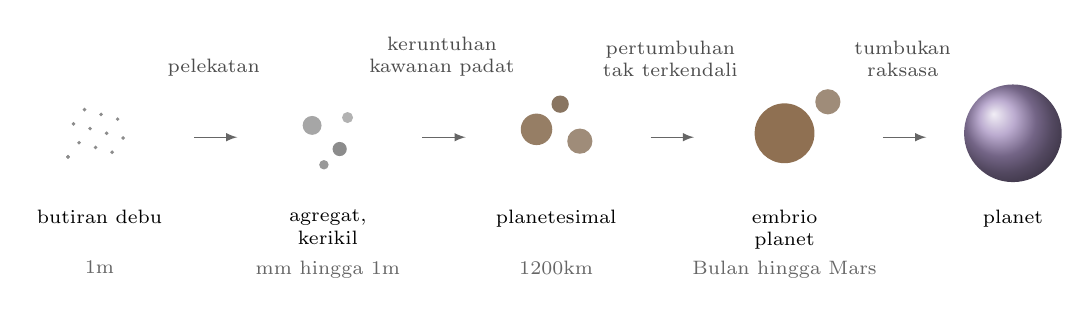
\begin{tikzpicture}[x=1cm, y=1cm, font=\scriptsize]
\foreach \x/\t/\s in {0/{butiran debu}/{\qty{1}{\micro m}},
  2.9/{agregat,\\kerikil}/{mm hingga \qty{1}{m}},
  5.8/{planetesimal}/{\qtyrange{1}{200}{km}},
  8.7/{embrio\\planet}/{Bulan hingga Mars},
  11.6/{planet}/{} } {
  \node[align=center, anchor=north] at (\x,-0.9) {\t};
  \node[align=center, anchor=north, black!60] at (\x,-1.55) {\s};
}
\foreach \i in {0,...,11} {\fill[black!45] ({-0.4+0.07*mod(\i*7,11)},{-0.35+0.06*mod(\i*5,11)}) circle (0.025);}
\fill[black!35] (2.7,0.05) circle (0.12); \fill[black!45] (3.05,-0.25) circle (0.09);
\fill[black!40] (2.85,-0.45) circle (0.06); \fill[black!30] (3.15,0.15) circle (0.07);
\fill[brown!55!black!70] (5.55,0) circle (0.2); \fill[brown!50!black!60] (6.1,-0.15) circle (0.16);
\fill[brown!45!black!70] (5.85,0.32) circle (0.11);
\fill[brown!60!black!80] (8.7,-0.05) circle (0.38); \fill[brown!50!black!60] (9.25,0.35) circle (0.16);
\shade[ball color=blue!45!brown!60] (11.6,-0.05) circle (0.62);
\foreach \x in {1.2,4.1,7.0,9.95} {\draw[-latex, black!60] (\x,-0.1) -- +(0.55,0);}
\node[align=center, anchor=south, black!70] at (1.45,0.55) {pelekatan};
\node[align=center, anchor=south, black!70] at (4.35,0.55) {keruntuhan\\kawanan padat};
\node[align=center, anchor=south, black!70] at (7.25,0.55) {pertumbuhan\\tak terkendali};
\node[align=center, anchor=south, black!70] at (10.2,0.55) {tumbukan\\raksasa};
\end{tikzpicture}

\par\smallskip{\small Dari debu menjadi planet di daerah planet-planet berbatu
(skema, tidak berskala). Butiran melekat menjadi agregat; kawanan kerikil runtuh
menjadi \omterm{def:b2:planet-formation-meteorites:planetesimal}{planetesimal}; gravitasi membuat sebagian \omterm{def:b2:planet-formation-meteorites:planetesimal}{planetesimal} tumbuh tak terkendali menjadi embrio, yang
akhirnya bergabung menjadi planet. Di luar \omterm{def:b2:planet-formation-meteorites:snow-line}{garis salju}, embrio tumbuh lebih besar dan dapat
menangkap gas. Ukuran menurut Chiang dan Youdin (2010) serta Lugaro dan kawan-kawan (2018).}
% ledger: cy10:growth, lugaro:cai
\end{omfigure}

Planet-planet hanya menyimpan sedikit ingatan tentang sejarah ini: planet-planet itu melebur,
bercampur, dan mengolah ulang materinya. Rekamannya tersimpan dalam benda-benda yang berhenti
tumbuh, yaitu asteroid, dan dalam pecahan-pecahannya yang mencapai Bumi.

\section{Meteorit}

\begin{definition}[Meteorit, meteorit jatuhan, meteorit temuan]
\label{def:b2:planet-formation-meteorites:fall-find}
Yang disebut \emph{meteorit}\index{meteorit} adalah benda padat alami dari antariksa yang
selamat melewati atmosfer dan mencapai tanah. Yang disebut
\emph{meteorit jatuhan}\index{meteorit jatuhan} adalah meteorit yang dikumpulkan setelah
kedatangannya teramati, biasanya sebagai bola api; yang disebut \emph{meteorit
temuan}\index{meteorit temuan} adalah meteorit yang dikenali di tanah tanpa kejatuhannya
pernah terlihat.
\end{definition}

Bumi menyapu jauh lebih banyak debu daripada batu. Menurut pengukuran di salju
dataran tinggi Antarktika, sekitar \qty{5200}{t} debu luar bumi mencapai
tanah setiap tahun sebagai mikrometeorit dan sferul lebur, dari sekitar
\qty{15000}{t} yang memasuki atmosfer, sebagian besar dilepaskan oleh komet dan sekitar
seperlima oleh asteroid. \omterm{def:b2:planet-formation-meteorites:fall-find}{Meteorit}, yaitu batu dan besi yang cukup besar untuk
dikenali satu per satu, lebih sedikit: katalog dunia memuat sekitar
\num{45000} \omterm{def:b2:planet-formation-meteorites:fall-find}{meteorit}, dan hanya \num{1107} di antaranya \omterm{def:b2:planet-formation-meteorites:fall-find}{meteorit jatuhan}.
% ledger: rojas21:flux, data:b4-meteorites

Perbedaan itu penting. \omterm{def:b2:planet-formation-meteorites:fall-find}{Meteorit jatuhan} dikumpulkan dalam hitungan hari, sebelum hujan dan
oksigen mengubahnya, dan setiap jenis \omterm{def:b2:planet-formation-meteorites:fall-find}{meteorit} yang jatuh terkumpul
sama rata; \omterm{def:b2:planet-formation-meteorites:fall-find}{meteorit temuan} mungkin telah tergeletak di tanah selama ribuan tahun, dan
peluangnya ditemukan bergantung pada rupanya dan tempat jatuhnya. Separuh dari semua
\omterm{def:b2:planet-formation-meteorites:fall-find}{meteorit temuan} berasal dari Antarktika (kotak di bawah), tempat pencarian dilakukan secara
sistematis. \omterm{def:b2:planet-formation-meteorites:fall-find}{Meteorit jatuhan} adalah sampel yang lebih adil dari apa yang tiba (gambar di bawah):
lebih dari empat dari lima adalah \omterm{def:b2:planet-formation-meteorites:chondrule}{kondrit}, tiga dari empat \omterm{def:b2:planet-formation-meteorites:chondrule}{kondrit} biasa.
% ledger: data:b4-meteorites

\begin{omfigure}
\begin{tikzpicture}
\begin{axis}[width=0.86\linewidth, height=6.3cm, ybar, bar width=7pt,
  xmin=0.4, xmax=9.6, ymin=0.1, ymax=200, ymode=log, log origin=infty,
  xtick={1,...,9}, xticklabels={biasa, berkarbon, enstatit, kondrit lain,
    HED, akondrit lain, besi, besi-batu, tak terklasifikasi},
  x tick label style={font=\scriptsize, rotate=30, anchor=north east, inner sep=1pt},
  tick label style={font=\scriptsize}, label style={font=\small},
  ylabel={bagian dari sampel (\%)}, legend pos=north east, xtick pos=bottom,
  legend style={font=\scriptsize, draw=black!30}, ymajorgrids, grid style={black!12}]
\addplot[fill=orange!70, draw=none] table[x=idx, y=falls_pct] {figdata/out/bachelor-2-meteorites-frac.dat};
\addlegendentry{jatuhan (\num{1107})}
\addplot[fill=blue!45, draw=none] table[x=idx, y=finds_pct] {figdata/out/bachelor-2-meteorites-frac.dat};
\addlegendentry{temuan (\num{44534})}
\end{axis}
\end{tikzpicture}

\par\smallskip{\small \omterm{def:b2:planet-formation-meteorites:fall-find}{Meteorit} menurut kelasnya, sebagai persentase \omterm{def:b2:planet-formation-meteorites:fall-find}{meteorit jatuhan} dan
\omterm{def:b2:planet-formation-meteorites:fall-find}{meteorit temuan} (skala logaritmik); HED: howardit, eukrit, dan diogenit. Data: ekspor NASA
dari Meteoritical Bulletin Database milik The Meteoritical Society
(\num{45641} \omterm{def:b2:planet-formation-meteorites:fall-find}{meteorit} yang sah).}
% ledger: data:b4-meteorites
\end{omfigure}

\begin{inthefield}[Mencari meteorit di es biru]
\begin{minipage}[t]{0.6\linewidth}\vspace{0pt}
Sebagian besar lembaran es Antarktika berupa salju putih, tetapi pada sekitar
\qty{1}{\percent} permukaannya, tempat pegunungan menghalangi aliran es,
sekitar \qty{5}{cm} es hilang setiap tahun dan tampaklah es biru yang terbuka. \omterm{def:b2:planet-formation-meteorites:fall-find}{Meteorit}
yang jatuh di salju di hulu, selama puluhan ribu tahun, terkubur,
terbawa di dalam es, dan muncul kembali ke permukaan di tempat es itu menyusut:
es biru adalah sebuah perangkap. Sejak pengumpulan sistematis dimulai pada pertengahan 1970-an,
tim-tim telah menemukan lebih dari \num{30000} spesimen dari lapangan semacam itu, dan dalam
katalog separuh dari semua \omterm{def:b2:planet-formation-meteorites:fall-find}{meteorit temuan} berasal dari selatan \ang{60}\,LS. Para pencari
menyeberangi es dalam barisan, berjalan kaki atau dengan mobil salju, dan setiap batu yang ditemukan
dikumpulkan, betapa pun biasa rupanya, agar koleksinya tidak berat sebelah
ke arah batu-batu yang mencolok. Setiap temuan difoto di tempatnya tergeletak, untuk mencatat
konteksnya, dan diberi nomor lapangan; kemudian temuan itu menerima nama resminya, yaitu
kode tiga huruf untuk lapangan es diikuti tahun musim pencarian dan
nomor urut. Di laboratorium kurasi, batu-batu itu dipecah dengan
alat baja nirkarat atau dipotong kering dengan gergaji pita; \omterm{def:b2:planet-formation-meteorites:chondrule}{kondrit berkarbon},
yang mungkin mengandung senyawa organik, memiliki lemari tersendiri sejak 1978.
\end{minipage}\hfill
\begin{minipage}[t]{0.37\linewidth}\vspace{0pt}
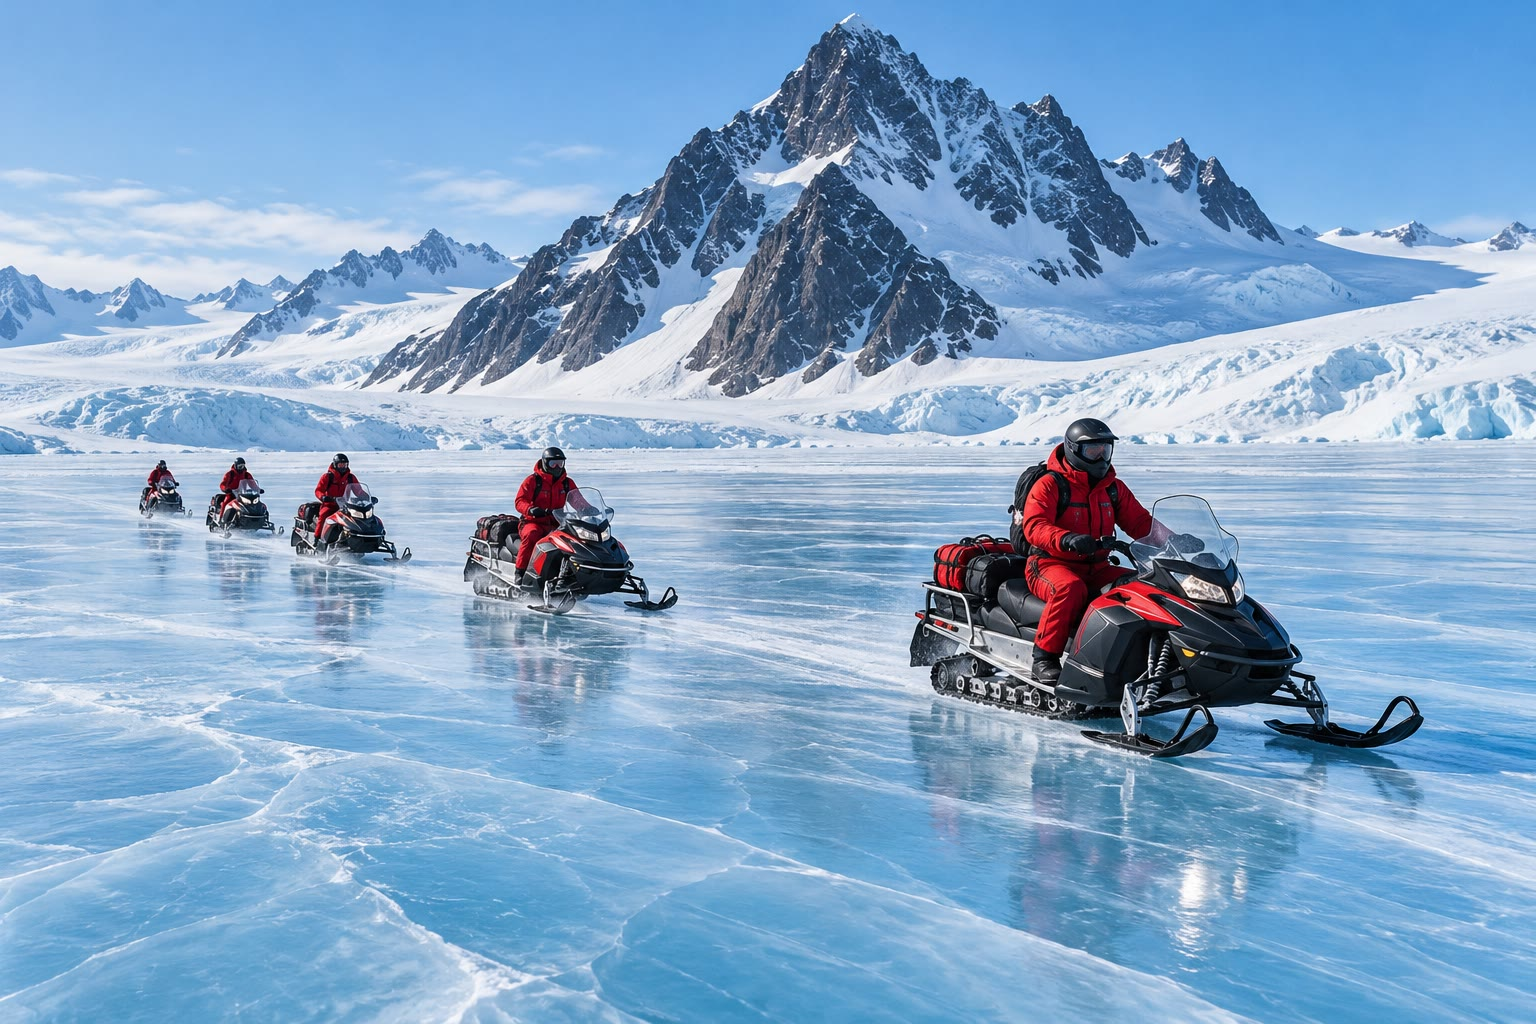
\includegraphics[width=\linewidth]{images/book4/ai/b2-blue-ice-search.jpg}

{\scriptsize Barisan pencari dengan mobil salju menyeberangi lapangan es biru di bawah
puncak berbatu (ilustrasi buatan AI).}
\end{minipage}
% ledger: folco06:blue-ice, data:b4-meteorites, nasa:antmet
\end{inthefield}

\subsection{Kondrit}

\begin{definition}[Kondrit, kondrit berkarbon, kondrul, CAI]
\label{def:b2:planet-formation-meteorites:chondrule}
Yang disebut \emph{kondrit}\index{kondrit} adalah \omterm{def:b2:planet-formation-meteorites:fall-find}{meteorit} batu yang tidak pernah melebur
setelah terhimpun, dan yang komposisinya, kecuali unsur-unsur yang paling volatil,
dekat dengan komposisi Matahari. Sebagian besar kondrit tersusun atas
\emph{kondrul}\index{kondrul}, yaitu tetesan bundar berukuran sepersepuluh milimeter hingga
sekitar satu sentimeter, dari batuan silikat yang membeku dari lelehan, yang tertanam dalam
matriks berbutir halus bersama butiran logam besi--nikel dan besi sulfida. Sebagian
kondrit mengandung \emph{inklusi yang kaya kalsium--aluminium}\index{inklusi kaya kalsium--aluminium}
(CAI), yaitu butiran putih tak beraturan dari mineral kalsium, aluminium,
dan titanium yang merupakan kondensat pertama nebula. Yang disebut
\emph{kondrit berkarbon}\index{kondrit berkarbon} adalah kondrit yang kaya
karbon, mineral yang mengandung air, dan matriks, yang kandungan unsur volatilnya
paling mendekati kandungan Matahari.
\end{definition}

\omterm{def:b2:planet-formation-meteorites:chondrule}{Kondrul} hanya cair selama beberapa menit dan mendingin selama beberapa jam hingga
beberapa hari: suatu pemanasan kilat yang singkat dan lokal di dalam nebula, yang penyebabnya
masih belum diketahui, melelehkan gumpalan debu, yang membeku menjadi tetesan sebelum tersapu
bersama debu dan logam ke dalam sebuah \omterm{def:b2:planet-formation-meteorites:planetesimal}{planetesimal}. \omterm{def:b2:planet-formation-meteorites:chondrule}{Kondrul} mengisi hingga \qty{90}{\percent} volume \omterm{def:b2:planet-formation-meteorites:fall-find}{meteorit} yang paling
primitif. CAI menyusun dari kurang dari \qty{1}{\percent}
\omterm{def:b2:planet-formation-meteorites:chondrule}{kondrit} biasa hingga lebih dari \qty{10}{\percent} sebagian \omterm{def:b2:planet-formation-meteorites:chondrule}{kondrit berkarbon}, dan CAI-CAI itu
terbentuk dalam selang sekitar seratus ribu tahun satu sama lain.
% ledger: gail:meteorites, cy10:growth, cy10:chondrules, gail:chondrite-table, lugaro:cai

\begin{omfigure}
\begin{minipage}[c]{0.5\linewidth}
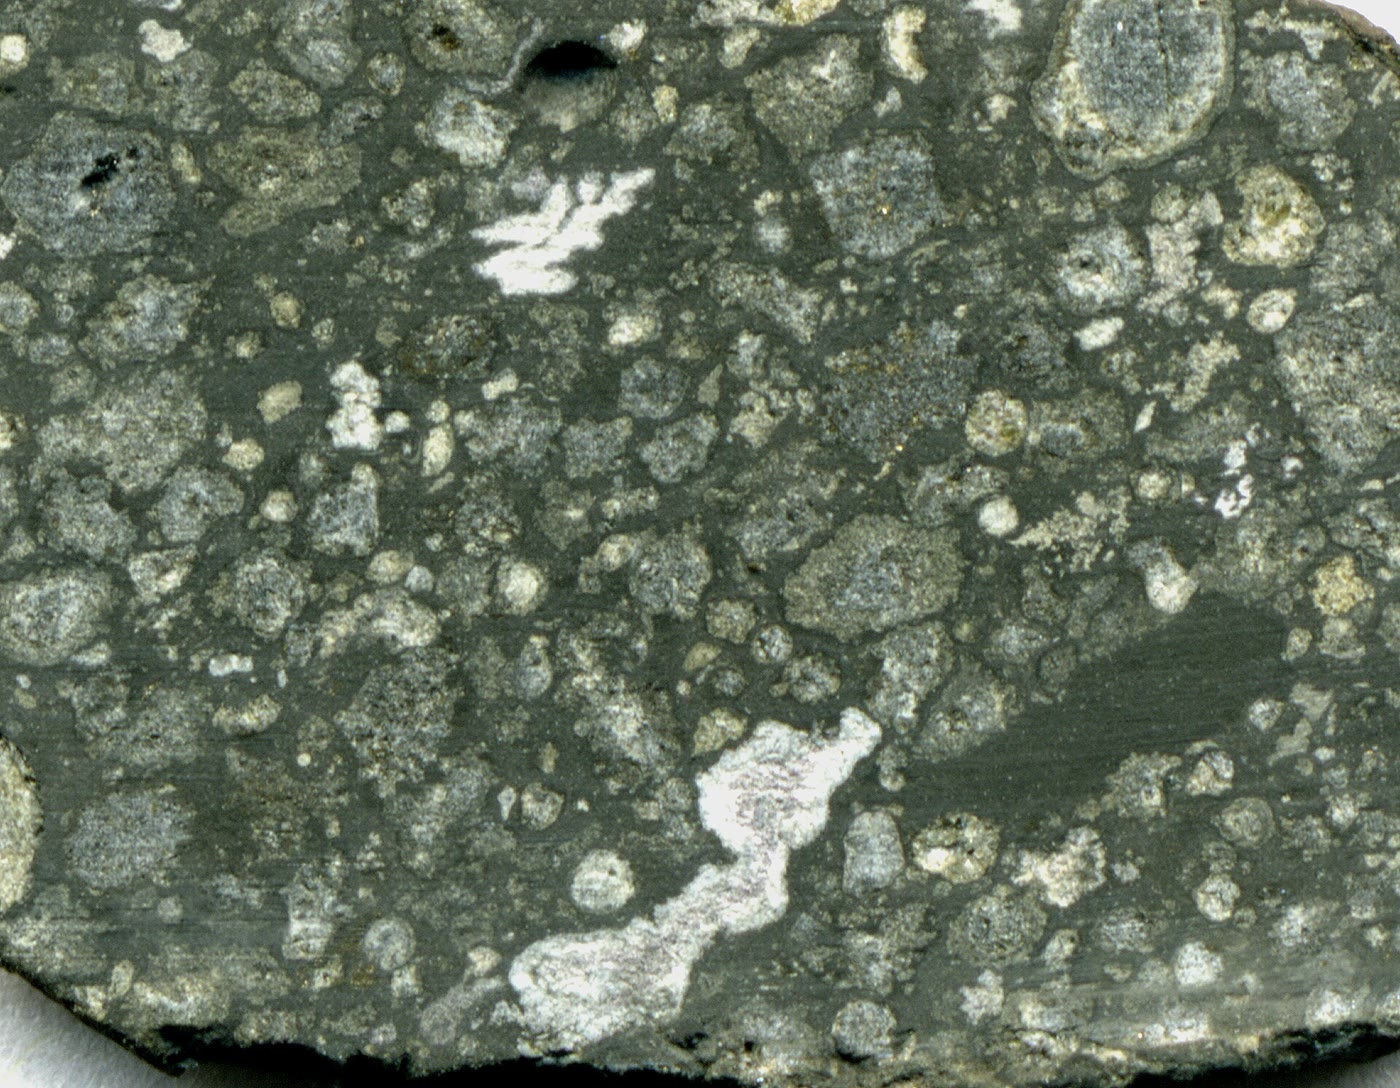
\includegraphics[width=\linewidth]{images/book4/b2-allende-chondrite.jpg}
\end{minipage}\hfill
\begin{minipage}[c]{0.46\linewidth}
{\small Permukaan potongan \omterm{def:b2:planet-formation-meteorites:chondrule}{kondrit berkarbon} Allende (kelas CV3), yang jatuh di
Meksiko utara pada tahun 1969: sekitar dua ton terkumpul. Butiran kelabu yang bundar adalah
\omterm{def:b2:planet-formation-meteorites:chondrule}{kondrul}; bercak putih tak beraturan adalah CAI; semen gelapnya adalah matriks. Medan
pandangnya selebar beberapa sentimeter. James St.\ John, CC BY 2.0.}
\end{minipage}
% ledger: data:b4-meteorites, gail:chondrite-table
\end{omfigure}

\omterm{def:b2:planet-formation-meteorites:chondrule}{Kondrit} terbagi menjadi kelompok-kelompok yang berbeda dalam ukuran dan kelimpahan
\omterm{def:b2:planet-formation-meteorites:chondrule}{kondrulnya}, kandungan logamnya, kandungan besi olivinnya, dan
proporsi matriksnya (tabel di bawah). \omterm{def:b2:planet-formation-meteorites:chondrule}{Kondrit} biasa H, L, dan LL
memiliki kandungan logam dan besi total yang tinggi, rendah, dan sangat rendah (perbandingan atom
Fe/Si \num{0.80}, \num{0.59}, dan \num{0.53}).
% ledger: gail:chondrite-table

\begin{table}[h]
\centering
\small
\begin{tabular}{lcccccc}
\hline
 & H & L & LL & CI & CM & CV\\
\hline
\omterm{def:b2:planet-formation-meteorites:chondrule}{kondrul} (\%\ vol.) & 60--80 & 60--80 & 60--80 & $\ll 1$ & 20 & 45\\
diameter rata-rata \omterm{def:b2:planet-formation-meteorites:chondrule}{kondrul} (mm) & 0.3 & 0.7 & 0.9 & --- & 0.3 & 1.0\\
CAI (\%\ vol.) & 0.1--1 & 0.1--1 & 0.1--1 & $\ll 1$ & 5 & 10\\
matriks (\%\ vol.) & 10--15 & 10--15 & 10--15 & $> 99$ & 70 & 40\\
logam besi--nikel (\%\ vol.) & 10 & 5 & 2 & 0 & 0.1 & 0--5\\
fayalit dalam olivin (\%\ mol) & 16--20 & 23--26 & 27--32 & & & \\
\omterm{def:b2:planet-formation-meteorites:type}{tipe petrologi} & 3--6 & 3--6 & 3--6 & 1 & 2 & 3\\
suhu tertinggi (K) & 1220 & 1220 & 1220 & 430 & 670 & 870\\
\hline
\end{tabular}
\caption{Sifat-sifat \omterm{def:b2:planet-formation-meteorites:chondrule}{kondrit} biasa (H, L, LL) dan tiga kelompok \omterm{def:b2:planet-formation-meteorites:chondrule}{kondrit
berkarbon}. Fayalit: anggota ujung besi olivin. Data: Gail dan kawan-kawan (2014).}
\label{tab:b2:planet-formation-meteorites:chondrites}
% ledger: gail:chondrite-table
\end{table}

\begin{definition}[Tipe petrologi]\label{def:b2:planet-formation-meteorites:type}
Yang disebut \emph{tipe petrologi}\index{tipe petrologi} sebuah \omterm{def:b2:planet-formation-meteorites:chondrule}{kondrit} adalah bilangan
dari 1 hingga 6 yang merekam apa yang terjadi padanya di dalam benda induknya: tipe 3 adalah
yang paling sedikit terubah; tipe 4 hingga 6 makin terpanaskan, \omterm{def:b2:planet-formation-meteorites:chondrule}{kondrulnya} makin kabur
dan mineralnya terkristalisasi ulang serta berkomposisi seragam; tipe 2 dan 1
makin terubah oleh air cair, yang mengubah mineralnya menjadi lempung.
\end{definition}

Baris terakhir tabel memberikan suhu tertinggi yang dicapai setiap kelompok:
hingga sekitar \qty{1220}{K} untuk \omterm{def:b2:planet-formation-meteorites:chondrule}{kondrit} biasa yang paling terpanaskan, tidak pernah lebih
dari \qty{430}{K} untuk \omterm{def:b2:planet-formation-meteorites:chondrule}{kondrit} CI, yang basah kuyup oleh air tetapi tidak pernah panas.
Pemanasannya, seperti ditunjukkan subbab terakhir, berasal dari dalam benda-benda induk itu.
% ledger: gail:chondrite-table

\subsection{Akondrit dan meteorit besi}

\begin{definition}[Akondrit, meteorit besi, meteorit besi-batu]
\label{def:b2:planet-formation-meteorites:classes}
Yang disebut \emph{akondrit}\index{akondrit} adalah \omterm{def:b2:planet-formation-meteorites:fall-find}{meteorit} batu yang mengkristal
dari lelehan atau terkristalisasi ulang pada suhu tinggi di dalam benda yang melebur,
sehingga tidak memiliki \omterm{def:b2:planet-formation-meteorites:chondrule}{kondrul}. Yang disebut \emph{meteorit besi}\index{meteorit besi} tersusun
terutama atas logam besi--nikel. Yang disebut \emph{meteorit
besi-batu}\index{meteorit besi-batu} tersusun atas logam dan silikat dalam jumlah yang
kira-kira sama.
\end{definition}

\omterm{def:b2:planet-formation-meteorites:fall-find}{Meteorit-meteorit} ini adalah pecahan benda-benda yang melebur dan terpisah: \omterm{def:b2:planet-formation-meteorites:classes}{akondrit} adalah
kerak dan mantelnya, \omterm{def:b2:planet-formation-meteorites:classes}{meteorit besi} inti logamnya, dan \omterm{def:b2:planet-formation-meteorites:classes}{meteorit besi-batu} berasal dari tempat
logam dan silikat bertemu. Keluarga \omterm{def:b2:planet-formation-meteorites:classes}{akondrit} terbesar, yaitu howardit,
eukrit, dan diogenit (HED), berupa basal dan batuan kaya piroksen, menyusun
\qty{5.5}{\percent} dari semua \omterm{def:b2:planet-formation-meteorites:fall-find}{meteorit jatuhan}. Sumbernya dilacak, melalui spektrum dan
orbitnya, ke asteroid Vesta, yang berdiameter sekitar \qty{525}{km}, dan wahana
Dawn, yang mencapai Vesta pada tahun 2011, mengonfirmasinya: kimia
dan mineralogi permukaan Vesta cocok dengan \omterm{def:b2:planet-formation-meteorites:fall-find}{meteorit} HED, sebuah cekungan
selebar \qty{500}{km} di dekat kutub selatannya menunjukkan tempat pecahan-pecahan itu terlepas
akibat tumbukan, dan medan gravitasinya menunjukkan inti besi berdiameter sekitar \qty{225}{km}.
Vesta melebur, hampir seluruhnya atau seluruhnya, pada awal sejarahnya. \omterm{def:b2:planet-formation-meteorites:classes}{Akondrit} lain berasal
dari Bulan dan dari Mars. \omterm{def:b2:planet-formation-meteorites:fall-find}{Meteorit-meteorit} dalam koleksi tampaknya berasal
dari sekitar seratus benda induk yang berbeda.
% ledger: data:b4-meteorites, nasa:vesta-dawn, gail:meteorites

\omterm{def:b2:planet-formation-meteorites:classes}{Meteorit besi} menyimpan rekaman cara intinya mendingin. Permukaan yang dipotong dan
dietsa asam memperlihatkan jalinan lempeng-lempeng yang bersilangan (gambar di bawah): pada suhu
tinggi logamnya berupa satu paduan besi dan nikel; pada pendinginan lambat, sebuah
paduan miskin nikel tumbuh berupa lempeng-lempeng di sepanjang bidang kristal asalnya,
dan makin lambat pendinginannya, makin lebar lempengnya. Diukur pada banyak \omterm{def:b2:planet-formation-meteorites:classes}{meteorit besi},
lebar lempeng memberikan laju pendinginan inti asalnya.
% ledger: gail:meteorites

\begin{omfigure}
\begin{minipage}[c]{0.5\linewidth}
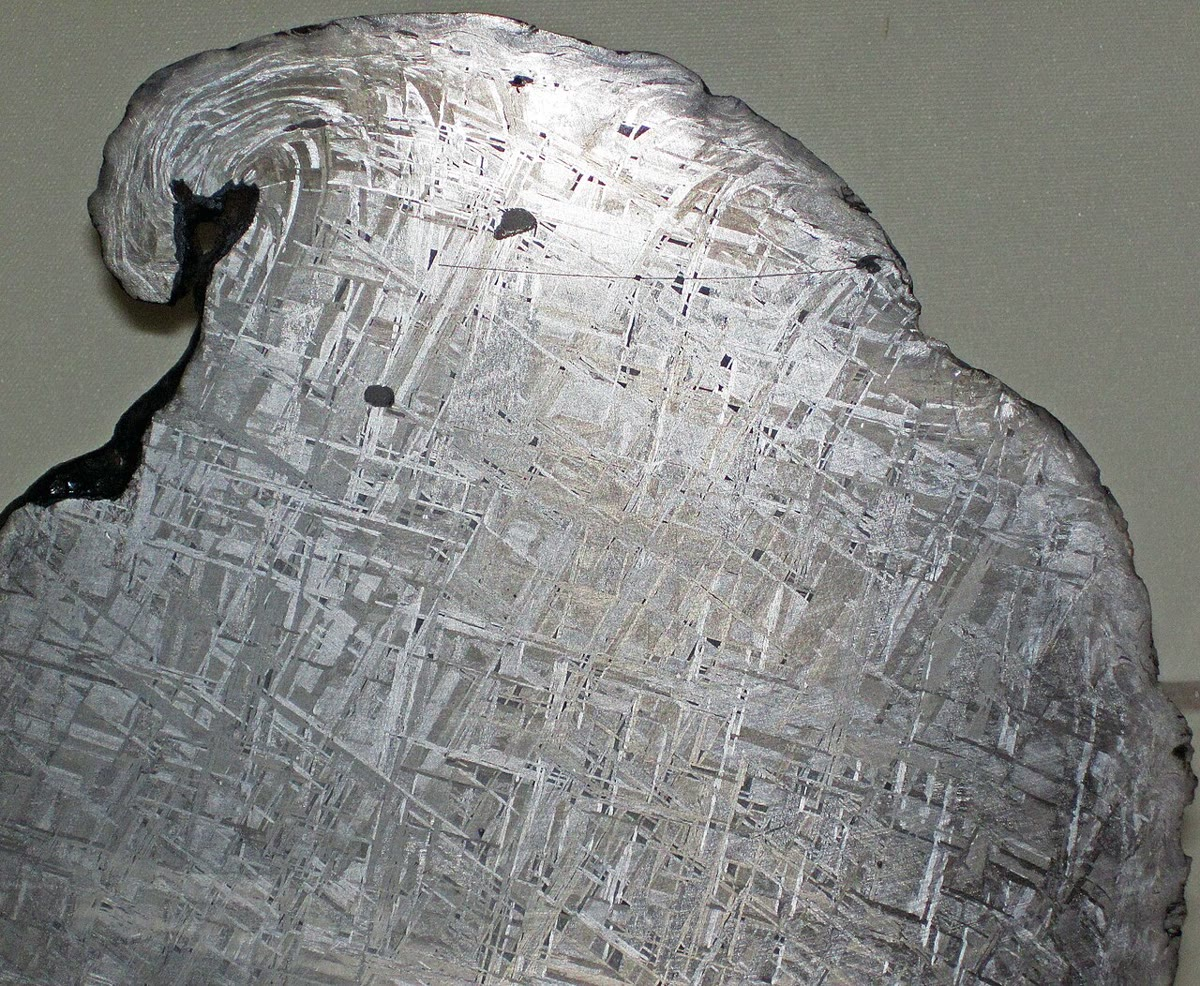
\includegraphics[width=\linewidth]{images/book4/b2-gibeon-widmanstatten.jpg}
\end{minipage}\hfill
\begin{minipage}[c]{0.46\linewidth}
{\small Permukaan sepotong \omterm{def:b2:planet-formation-meteorites:classes}{meteorit besi} Gibeon, yang ditemukan di Namibia, setelah dipotong,
dipoles, dan dietsa asam: jalinan lempeng paduan besi--nikel yang bersilangan (pola
Widmanstätten) tumbuh ketika inti logam benda induknya mendingin perlahan. James St.\ John,
CC BY 2.0.}
\end{minipage}
% ledger: data:b4-meteorites
\end{omfigure}

\section{Menentukan umur Tata Surya}

Umur Tata Surya adalah umur zat padatnya yang tertua. Isokron uranium--timbal
CAI, yang dibangun seperti dalam volume Tahun 1, memberikan \qtyrange{4567}{4568}{\Ma};
CAI terbentuk dalam selang sekitar \qty{0.1}{Ma} satu sama lain, waktu yang cukup singkat
sehingga umurnya dapat dianggap sebagai kelahiran Matahari. Peristiwa-peristiwa dalam
beberapa juta tahun berikutnya, yaitu pembentukan \omterm{def:b2:planet-formation-meteorites:chondrule}{kondrul} serta penghimpunan dan
peleburan benda-benda pertama, paling baik ditentukan umurnya relatif terhadap CAI, dengan jam-jam
yang berjalan cepat dan berhenti lebih awal.
% ledger: lugaro:cai

\begin{definition}[Radionuklida berumur pendek]
\label{def:b2:planet-formation-meteorites:slr}
Yang disebut \emph{radionuklida berumur pendek}\index{radionuklida berumur pendek} adalah
nuklida radioaktif dengan waktu paruh kira-kira \num{0.1} hingga \qty{100}{Ma},
yang ada ketika Tata Surya terbentuk dan kini sudah punah, yang kehadirannya dahulu
ditunjukkan oleh kelebihan anaknya dalam mineral-mineral yang kaya akan
unsurnya.
\end{definition}

Yang paling terkenal adalah aluminium-26, yang meluruh menjadi magnesium-26 dengan waktu paruh
\qty{0.717}{Ma} (umur rata-rata \qty{1.035}{Ma}). Ketika CAI terbentuk, satu
dari sekitar \num{19000} atom aluminium adalah aluminium-26: perbandingan
$\ce{^{26}Al}/\ce{^{27}Al}$ bernilai $(5.23 \pm 0.13)\times10^{-5}$, yaitu nilai
\emph{kanonik}. Nuklida berumur pendek lainnya meliputi rentang yang lebih panjang (tabel
di bawah).
% ledger: lugaro:al26, lugaro:slr-table

\begin{table}[h]
\centering
\small
\begin{tabular}{lllcc}
\hline
nuklida & anak & acuan & waktu paruh (Ma) & perbandingan awal\\
\hline
\ce{^{26}Al} & \ce{^{26}Mg} & \ce{^{27}Al} & 0.717 & $5.23\times10^{-5}$\\
\ce{^{60}Fe} & \ce{^{60}Ni} & \ce{^{56}Fe} & 2.62 & $1.0\times10^{-8}$\\
\ce{^{53}Mn} & \ce{^{53}Cr} & \ce{^{55}Mn} & 3.74 & $7\times10^{-6}$\\
\ce{^{107}Pd} & \ce{^{107}Ag} & \ce{^{108}Pd} & 6.5 & $6.6\times10^{-5}$\\
\ce{^{182}Hf} & \ce{^{182}W} & \ce{^{180}Hf} & 8.90 & $1.02\times10^{-4}$\\
\ce{^{129}I} & \ce{^{129}Xe} & \ce{^{127}I} & 15.7 & $1.28\times10^{-4}$\\
\hline
\end{tabular}
\caption{Beberapa \omterm{def:b2:planet-formation-meteorites:slr}{radionuklida berumur pendek} Tata Surya awal, anak
stabilnya, isotop stabil unsur yang sama yang dipakai sebagai acuan, waktu
paruhnya, dan perbandingannya terhadap acuan ketika CAI terbentuk. Data: Lugaro dan
kawan-kawan (2018).}
\label{tab:b2:planet-formation-meteorites:slr}
% ledger: lugaro:al26, lugaro:slr-table
\end{table}

\begin{proposition}[Umur relatif dari nuklida punah]
\label{prop:b2:planet-formation-meteorites:relative-age}
Jika perbandingan sebuah nuklida berumur pendek terhadap isotop acuannya bernilai $R_0$
di mana-mana ketika CAI terbentuk, dan ternyata bernilai $R$ dalam suatu objek ketika
objek itu terbentuk, maka objek itu terbentuk
\[
  \Delta t = \tau \ln\frac{R_0}{R}
\]
setelah CAI, dengan $\tau$ adalah umur rata-rata nuklida itu. Galat
$\delta R$ pada $R$ menghasilkan galat $\tau\,\delta R/R$ pada $\Delta t$.
\end{proposition}

\begin{proof}
Isotop acuannya stabil, sehingga perbandingan itu meluruh seperti nuklida radioaktif
itu sendiri: $R = R_0 e^{-\Delta t/\tau}$. Dengan mengambil logaritma,
$\Delta t = \tau\ln(R_0/R)$. Dengan menurunkannya, $\mathrm d(\Delta t) =
-\tau\,\mathrm dR/R$.
\end{proof}

Jadi galat relatif \qty{10}{\percent} pada perbandingan itu bernilai
\qty{0.1}{Ma} untuk aluminium-26, tetapi \qty{0.54}{Ma} untuk mangan-53 dan
\qty{1.3}{Ma} untuk hafnium-182: setiap jam hanya teliti dalam rentang beberapa umur
rata-ratanya sendiri, dan jam yang tepat bergantung pada peristiwanya. Perbandingan $R$ dalam
sebuah objek dibaca dari mineral-mineralnya.
% ledger: lugaro:al26, lugaro:slr-table

\begin{proposition}[Isokron aluminium--magnesium]
\label{prop:b2:planet-formation-meteorites:al-mg}
Misalkan beberapa mineral dari satu objek terbentuk bersama pada waktu $\Delta t$ dengan
komposisi isotop magnesium yang sama, $(\ce{^{26}Mg}/\ce{^{24}Mg})_0$, tetapi
perbandingan $\ce{^{27}Al}/\ce{^{24}Mg}$ yang berbeda, dan sejak itu tetap tertutup. Kini mineral-mineral itu
terletak pada garis lurus
\[
  \frac{\ce{^{26}Mg}}{\ce{^{24}Mg}}
  = \left(\frac{\ce{^{26}Mg}}{\ce{^{24}Mg}}\right)_0
  + R\,\frac{\ce{^{27}Al}}{\ce{^{24}Mg}},
\]
yang kemiringannya adalah perbandingan $R = \ce{^{26}Al}/\ce{^{27}Al}$ objek itu ketika
terbentuk.
\end{proposition}

\begin{proof}
Setiap atom aluminium-26 yang ada saat pembentukan sejak itu telah menjadi
atom magnesium-26, sehingga sebuah mineral memperoleh
$\ce{^{26}Al}_{\text{awal}} = R\,\ce{^{27}Al}$ atom magnesium-26, karena aluminium-27
stabil. Membaginya dengan jumlah atom magnesium-24, yang tidak berubah,
menghasilkan garis itu.
\end{proof}

Mineral yang kaya aluminium dan miskin magnesium, seperti plagioklas, memperlihatkan kelebihan
magnesium-26 yang besar; olivin, yang hampir tanpa aluminium, tidak memperlihatkannya. Dengan cara inilah
urutan waktu Tata Surya awal disusun: CAI lebih dulu; \omterm{def:b2:planet-formation-meteorites:chondrule}{kondrul} dalam
beberapa juta tahun berikutnya, dengan bukti dari \omterm{def:b2:planet-formation-meteorites:chondrule}{kondrul} yang menetapkan
umur cakram gas kurang dari lima juta tahun; benda-benda induk
\omterm{def:b2:planet-formation-meteorites:chondrule}{kondrit} terhimpun setelah \omterm{def:b2:planet-formation-meteorites:chondrule}{kondrul-kondrulnya} yang termuda. Diogenit,
batuan mantel Vesta, mulai mengkristal dalam sekitar satu juta tahun setelah
CAI, dan inti Vesta terbentuk dalam satu hingga
empat juta tahun pertama: \omterm{def:b2:planet-formation-meteorites:classes}{meteorit besi} dan \omterm{def:b2:planet-formation-meteorites:classes}{akondrit} lebih tua daripada banyak
\omterm{def:b2:planet-formation-meteorites:chondrule}{kondrit}.
% ledger: lugaro:cai, gail:vesta, gail:meteorites

\section{Panas dari aluminium-26 dan peleburan pertama}

Dari mana datangnya panas yang melebur Vesta dan memetamorfosis \omterm{def:b2:planet-formation-meteorites:chondrule}{kondrit}
biasa? Model dan \omterm{def:b2:planet-formation-meteorites:fall-find}{meteorit} sepakat bahwa dalam benda-benda paling awal
sumber utamanya adalah peluruhan aluminium-26. Dalam batuan berkomposisi kondritik, aluminium-26 pada awalnya membawa
\qty{5}{MJ} per kilogram yang siap dilepaskan dalam beberapa juta tahun:
cukup untuk memanaskan batuan sebesar ribuan kelvin, seandainya panasnya tidak dapat lolos.
% ledger: lugaro:heat, lugaro:melting

\begin{proposition}[Pemanasan planetesimal oleh aluminium-26]
\label{prop:b2:planet-formation-meteorites:heating}
Batuan yang menerima daya radioaktif $H_0 e^{-t/\tau}$ per kilogram, berkapasitas
kalor jenis $c$, dan tidak kehilangan panas, menghangat setelah akresinya pada
waktu $t_a$ sebagai
\[
  T(t) = T_0 + \frac{H_0\tau}{c}\left(e^{-t_a/\tau} - e^{-t/\tau}\right),
\]
dan mendekati suhu puncak
$T_{\max} = T_0 + (H_0\tau/c)\,e^{-t_a/\tau}$. Suhu kritis
$T_c > T_0$ hanya tercapai jika benda itu terakresi sebelum
\[
  t_a^* = \tau\ln\frac{H_0\tau}{c\,(T_c - T_0)}.
\]
\end{proposition}

\begin{proof}
Tanpa kehilangan panas, $c\,\mathrm dT/\mathrm dt = H_0 e^{-t/\tau}$. Mengintegrasikan dari
$t_a$, tempat $T = T_0$, menghasilkan
$c\,(T - T_0) = H_0\tau\,(e^{-t_a/\tau} - e^{-t/\tau})$, yang mendekati
$H_0\tau e^{-t_a/\tau}$ ketika $t \to \infty$. Menetapkan $T_{\max} = T_c$ dan menyelesaikannya
untuk $t_a$ menghasilkan $t_a^*$; untuk akresi yang lebih awal, puncaknya lebih tinggi.
\end{proof}

Sebuah model benda induk \omterm{def:b2:planet-formation-meteorites:chondrule}{kondrit} biasa memakai
$H_0 = \qty{1.9e-7}{W.kg^{-1}}$, $c = \qty{837}{J.kg^{-1}.K^{-1}}$, dan
$T_0 = \qty{250}{K}$. Maka $H_0\tau/c$ sekitar \qty{7400}{K}. Tiga
suhu itu penting: di dekat \qty{750}{K} batuan berpori mulai tersinter menjadi batuan
yang kompak; di dekat \qty{1200}{K} logam dan besi sulfida mulai melebur
bersama; di dekat \qty{1700}{K} silikat terakhir melebur. Benda yang terakresi
sebelum \qty{1.7}{Ma} melebur seluruhnya; sebelum \qty{2.1}{Ma} logam dan sulfidanya
melebur dan dapat tenggelam membentuk inti; hingga sekitar \qty{2.8}{Ma} benda itu setidaknya
tersinter dan termetamorfosis; benda-benda yang lebih muda tetap dingin (gambar di bawah).
% ledger: gail:params, gail:temps, lugaro:al26

\begin{omfigure}
\begin{tikzpicture}
\begin{axis}[omrecord, name=left, width=0.45\linewidth, height=6.0cm,
  xmin=0, xmax=8, ymin=0, ymax=2300,
  xlabel={waktu setelah CAI (Ma)}, ylabel={suhu (K)},
  tick label style={font=\scriptsize}, label style={font=\small}]
\addplot[black!45, densely dashed, domain=0:8, samples=2] {750};
\addplot[black!45, densely dashed, domain=0:8, samples=2] {1200};
\addplot[black!45, densely dashed, domain=0:8, samples=2] {1700};
\addplot[thick, red!75!black] table[x=t_Myr, y=T_K] {figdata/out/bachelor-2-al26-ta15.dat};
\addplot[thick, orange!80!black] table[x=t_Myr, y=T_K] {figdata/out/bachelor-2-al26-ta20.dat};
\addplot[thick, teal!70!black] table[x=t_Myr, y=T_K] {figdata/out/bachelor-2-al26-ta25.dat};
\addplot[thick, blue!70!black] table[x=t_Myr, y=T_K] {figdata/out/bachelor-2-al26-ta30.dat};
\node[font=\tiny, red!75!black, anchor=south east] at (axis cs:7.9,1995) {$t_a = \qty{1.5}{Ma}$};
\node[font=\tiny, orange!80!black, anchor=south east] at (axis cs:7.9,1325) {2};
\node[font=\tiny, teal!70!black, anchor=south east] at (axis cs:7.9,915) {2.5};
\node[font=\tiny, blue!70!black, anchor=north east] at (axis cs:7.9,650) {3};
\node[font=\tiny, black!60, anchor=south west] at (axis cs:0.1,1700) {silikat melebur};
\node[font=\tiny, black!60, anchor=south west] at (axis cs:0.1,1200) {Fe--FeS melebur};
\node[font=\tiny, black!60, anchor=south west] at (axis cs:0.1,750) {sinter};
\end{axis}
\begin{axis}[omrecord, at={(left.east)}, anchor=west, xshift=2.1cm, width=0.45\linewidth,
  height=6.0cm, xmin=0, xmax=4, ymin=0, ymax=8000,
  xlabel={waktu akresi $t_a$ (Ma)}, ylabel={suhu puncak (K)},
  tick label style={font=\scriptsize}, label style={font=\small},
  scaled y ticks=false, yticklabel style={/pgf/number format/1000 sep={\,}}]
\addplot[black!45, densely dashed, domain=0:4, samples=2] {750};
\addplot[black!45, densely dashed, domain=0:4, samples=2] {1200};
\addplot[black!45, densely dashed, domain=0:4, samples=2] {1700};
\addplot[thick, black] table[x=ta_Myr, y=Tpeak_K] {figdata/out/bachelor-2-al26-peak.dat};
\draw[black!60] (axis cs:1.69,0) -- (axis cs:1.69,1700);
\draw[black!60] (axis cs:2.13,0) -- (axis cs:2.13,1200);
\node[font=\tiny, black!70, anchor=south] at (axis cs:2.0,4500) {\qty{1.7}{Ma}};
\draw[black!50, -latex] (axis cs:2.0,4450) -- (axis cs:1.71,1800);
\node[font=\tiny, black!70, anchor=south] at (axis cs:2.9,3300) {\qty{2.1}{Ma}};
\draw[black!50, -latex] (axis cs:2.9,3250) -- (axis cs:2.16,1300);
\end{axis}
\end{tikzpicture}

\par\smallskip{\small Pemanasan bagian dalam benda kondritik oleh aluminium-26 tanpa
kehilangan panas (proposisi di atas; $H_0 = \qty{1.9e-7}{W.kg^{-1}}$,
$c = \qty{837}{J.kg^{-1}.K^{-1}}$, $T_0 = \qty{250}{K}$, $\tau = \qty{1.035}{Ma}$).
Kiri: suhu terhadap waktu untuk benda yang terakresi 1.5, 2, 2.5, dan \qty{3}{Ma}
setelah CAI. Kanan: suhu puncak terhadap waktu akresi; benda yang terakresi
sebelum \qty{1.7}{Ma} melebur, sebelum \qty{2.1}{Ma} logam dan sulfidanya melebur.
Benda yang sebenarnya memakai sebagian panasnya untuk melebur, yang membatasi suhunya, dan kehilangan
panas di dekat permukaannya. Nilai model: Gail dan kawan-kawan (2014).}
% ledger: gail:params, gail:temps, lugaro:al26
\end{omfigure}

Proposisi itu mengabaikan kehilangan panas, yang hanya berlaku jauh di dalam benda besar.
Panas berdifusi sejauh $\sqrt{\kappa t}$ dalam waktu $t$, dengan
$\kappa$ adalah difusivitas termal batuan: dengan nilai-nilai model itu,
sekitar \qty{5}{km} dalam satu umur rata-rata aluminium-26 (\cref{exo:b2:planet-formation-meteorites:12}). Benda yang jauh
lebih kecil daripada ini kehilangan panasnya secepat ia menghasilkannya; model terperinci menunjukkan
bahwa benda berdiameter lebih dari \qtyrange{10}{20}{km} dapat melebur.
% ledger: gail:params, lugaro:melting

\begin{definition}[Diferensiasi planet]
\label{def:b2:planet-formation-meteorites:differentiation}
Yang disebut \emph{diferensiasi planet}\index{diferensiasi planet} adalah
pemisahan sebuah benda, yang pernah cair atau sebagian cair, menjadi lapisan-lapisan yang berbeda
komposisi dan massa jenisnya: inti logam, mantel silikat, dan kerak yang tersusun atas
lelehan-lelehan terakhir.
\end{definition}

Dengan demikian, \omterm{def:b2:planet-formation-meteorites:fall-find}{meteorit} merekam dua jenis benda awal. Benda yang terbentuk dalam
sekitar dua juta tahun pertama memiliki cukup aluminium-26 untuk melebur dan
terdiferensiasi: intinya adalah \omterm{def:b2:planet-formation-meteorites:classes}{meteorit besi}, kerak dan mantelnya
\omterm{def:b2:planet-formation-meteorites:classes}{akondrit}, dan Vesta yang tersisa. Benda yang terbentuk kemudian tetap menjadi
\omterm{def:b2:planet-formation-meteorites:chondrule}{kondrit}, yang dipanaskan dari dalam sampai tingkat yang ditentukan oleh waktu kelahirannya dan oleh
kedalaman setiap pecahannya: yang terdalam menjadi tipe 6, yang terdangkal tetap
tipe 3. Bumi sendiri, yang dibangun dari embrio dan \omterm{def:b2:planet-formation-meteorites:planetesimal}{planetesimal} kedua jenis itu dan
dihantam tumbukan raksasa, terdiferensiasi menjadi inti, mantel, dan keraknya.
% ledger: gail:meteorites, gail:vesta, gail:temps

\section{Latihan}

\begin{exercise}[$\star$]\label{exo:b2:planet-formation-meteorites:1}
Dalam \omterm{def:b2:planet-formation-meteorites:nebula}{nebula surya} bermassa minimum, hitunglah kerapatan permukaan gas pada
\qty{1}{au} dan pada \qty{5.2}{au}, serta kerapatan permukaan zat padat pada
\qty{1}{au} (hanya batuan, $Z_{\mathrm{rel}} = 0.33$) dan pada \qty{5.2}{au} (semua es
telah mengembun, $Z_{\mathrm{rel}} = 1$). Berapa kali lebih berat gas daripada zat padat
pada \qty{5.2}{au}?
% ledger: cy10:mmsn
\end{exercise}

\begin{exercise}[$\star$]\label{exo:b2:planet-formation-meteorites:2}
Dengan menggunakan gambar \omterm{def:b2:planet-formation-meteorites:condensation}{suhu kondensasi}, urutkan aluminium, natrium,
magnesium, besi, belerang, dan oksigen (sebagai es air) dari yang pertama mengembun hingga
yang terakhir, dan berikan kelompok kevolatilan masing-masing. Unsur mana yang kamu duga
diperkaya dalam CAI, dan mana yang terkuras di Bumi dibandingkan dengan Matahari?
% ledger: lodders:tc-table, lodders:groups
\end{exercise}

\begin{exercise}[$\star$]\label{exo:b2:planet-formation-meteorites:3}
Katalog mencantumkan \num{1107} \omterm{def:b2:planet-formation-meteorites:fall-find}{meteorit jatuhan}, 856 di antaranya \omterm{def:b2:planet-formation-meteorites:chondrule}{kondrit} biasa dan
49 \omterm{def:b2:planet-formation-meteorites:classes}{meteorit besi}, serta \num{44534} \omterm{def:b2:planet-formation-meteorites:fall-find}{meteorit temuan}, \num{38647} di antaranya \omterm{def:b2:planet-formation-meteorites:chondrule}{kondrit} biasa,
\num{1020} \omterm{def:b2:planet-formation-meteorites:classes}{meteorit besi}, dan \num{22096} berasal dari selatan \ang{60}\,LS. Hitunglah
bagian \omterm{def:b2:planet-formation-meteorites:chondrule}{kondrit} biasa dan \omterm{def:b2:planet-formation-meteorites:classes}{meteorit besi} di antara \omterm{def:b2:planet-formation-meteorites:fall-find}{meteorit jatuhan} dan di antara \omterm{def:b2:planet-formation-meteorites:fall-find}{meteorit temuan},
serta bagian \omterm{def:b2:planet-formation-meteorites:fall-find}{meteorit temuan} Antarktika. Sampel mana yang akan kamu gunakan untuk menaksir
proporsi kedatangan kelas-kelas itu di Bumi, dan mengapa?
% ledger: data:b4-meteorites
\end{exercise}

\begin{exercise}[$\star$]\label{exo:b2:planet-formation-meteorites:4}
Mineral-mineral sebuah objek memberikan perbandingan awal
$\ce{^{26}Al}/\ce{^{27}Al} = \num{1.0e-5}$. Berapa lama setelah CAI objek itu terbentuk?
Ambil $R_0 = \num{5.23e-5}$ dan umur rata-rata \qty{1.035}{Ma}.
% ledger: lugaro:al26
\end{exercise}

\begin{exercise}[$\star\star$]\label{exo:b2:planet-formation-meteorites:5}
Dengan menggunakan \cref{prop:b2:planet-formation-meteorites:disc-mass} dengan
$\Sigma_1 = \qty{2.2e4}{kg.m^{-2}}$ pada \qty{1}{au} (\qty{1}{au} $=
\qty{1.496e11}{m}$, $M_\odot = \qty{1.989e30}{kg}$), hitunglah massa
nebula bermassa minimum di dalam \qty{30}{au} dan di dalam \qty{100}{au}, dalam massa
Matahari. Bandingkan dengan cakram yang teramati, \numrange{0.001}{0.1} massa Matahari.
% ledger: cy10:mmsn
\end{exercise}

\begin{exercise}[$\star\star$]\label{exo:b2:planet-formation-meteorites:6}
Dalam cakram pasif $T = \qty{120}{K}\,(r/\qty{1}{au})^{-3/7}$, tentukan tempat es
air (\qty{182}{K}) dan es metana (\qty{41}{K}) menjadi stabil. Sebutir debu dalam cahaya
Matahari langsung mencapai \qty{182}{K} pada \qty{2.3}{au}. Mengapa kedua taksiran
\omterm{def:b2:planet-formation-meteorites:snow-line}{garis salju} itu berbeda, dan mana yang berlaku bagi benda-benda yang membangun planet?
% ledger: cy10:passive, lodders:phases
\end{exercise}

\begin{exercise}[$\star\star$]\label{exo:b2:planet-formation-meteorites:7}
Hitunglah massa isolasi, dengan $b = 5$, sebuah embrio pada \qty{1}{au} dalam
nebula bermassa minimum ($\Sigma_p = \qty{10.9}{g.cm^{-2}}$), dan pada \qty{5.2}{au}
di luar \omterm{def:b2:planet-formation-meteorites:snow-line}{garis salju} ($\Sigma_p = \qty{2.78}{g.cm^{-2}}$), dalam massa Bumi
($M_\oplus = \qty{5.972e24}{kg}$, $M_\odot = \qty{1.989e30}{kg}$). Menjadi berapa
massa itu pada \qty{5.2}{au} dalam cakram dengan zat padat \num{3.5} kali lebih banyak?
% ledger: cy10:isolation, cy10:mmsn, earth:mass
\end{exercise}

\begin{exercise}[$\star\star$]\label{exo:b2:planet-formation-meteorites:8}
Batuan berkomposisi CI mengandung \num{1.01e16} atom aluminium-26 per gram ketika
CAI terbentuk, dan setiap peluruhan meninggalkan panas \qty{5.00e-13}{J}. Hitunglah
panas yang dilepaskan per kilogram selama seluruh peluruhan, dan kenaikan suhu yang
akan dihasilkannya dengan $c = \qty{837}{J.kg^{-1}.K^{-1}}$ dan tanpa kehilangan panas. Berapa kali
lebih besar panas itu daripada panas yang diperlukan untuk menghangatkan batuan dari \num{250} hingga
\qty{1700}{K}?
% ledger: lugaro:heat, gail:params
\end{exercise}

\begin{exercise}[$\star\star$]\label{exo:b2:planet-formation-meteorites:9}
Selama seluruh peluruhannya, aluminium-26 melepaskan \qty{5.07e10}{erg} per gram batuan
CI dan besi-60 \qty{7.49e7}{erg} per gram. Hitunglah perbandingan kedua
energi itu. Waktu paruh besi-60 adalah \qty{2.62}{Ma}: hitunglah umur rata-ratanya,
dan perbandingan kedua daya pemanasan awal, yaitu energi dibagi umur rata-rata.
% ledger: lugaro:heat, lugaro:slr-table, lugaro:al26
\end{exercise}

\begin{exercise}[$\star\star\star$]\label{exo:b2:planet-formation-meteorites:10}
Dengan hasil \cref{exo:b2:planet-formation-meteorites:9}, tentukan waktu setelah besi-60 memanaskan batuan
lebih cepat daripada aluminium-26. Dapatkah besi-60 melebur benda yang terakresi
selambat itu? (Bandingkan energi yang masih harus dilepaskannya saat itu dengan
\qty{1.2e6}{J.kg^{-1}} yang diperlukan untuk menghangatkan batuan dari \num{250} hingga \qty{1700}{K}.)
% ledger: lugaro:heat, lugaro:slr-table, lugaro:al26
\end{exercise}

\begin{exercise}[$\star\star\star$]\label{exo:b2:planet-formation-meteorites:11}
Dengan $H_0 = \qty{1.9e-7}{W.kg^{-1}}$, $\tau = \qty{1.035}{Ma}$,
$c = \qty{837}{J.kg^{-1}.K^{-1}}$, dan $T_0 = \qty{250}{K}$ (satu tahun
\qty{3.156e7}{s}), hitunglah waktu akresi paling lambat agar pusat sebuah
benda besar mencapai \qty{1200}{K} dan \qty{1700}{K}. Beberapa pengukuran menunjukkan bahwa
aluminium-26 awal hanya separuh nilai kanoniknya di beberapa bagian cakram:
seberapa jauh kedua waktu itu akan bergeser? Tunjukkan bahwa pergeseran itu tidak bergantung pada
suhu kritisnya.
% ledger: gail:params, gail:temps, lugaro:al26
\end{exercise}

\begin{exercise}[$\star\star\star$]\label{exo:b2:planet-formation-meteorites:12}
Batuan berkonduktivitas \qty{2.1}{W.m^{-1}.K^{-1}}, bermassa jenis
\qty{3300}{kg.m^{-3}}, dan berkapasitas kalor jenis \qty{837}{J.kg^{-1}.K^{-1}} memiliki
difusivitas termal $\kappa = k/(\rho c)$. Hitunglah nilainya, serta jarak
$\sqrt{\kappa\tau}$ yang ditempuh difusi panas dalam satu umur rata-rata aluminium-26.
Jelaskan mengapa proposisi pemanasan berlaku untuk pusat benda berdiameter
\qty{100}{km} tetapi tidak untuk benda berdiameter \qty{2}{km}, dan bandingkan dengan
benda terkecil yang dapat melebur, berdiameter \qtyrange{10}{20}{km}.
% ledger: gail:params, lugaro:melting, lugaro:al26
\end{exercise}

\section{Soal: Batu yang jatuh di danau beku}

\begin{problem}[{Soal akhir pekan --- mengklasifikasikan batu yang baru jatuh, menentukan umur
kondrulnya dengan aluminium-26, dan mencari seberapa panas benda induknya}]
\label{pb:b2:planet-formation-meteorites:1}
% values: calc/ch02.py
% ledger: data:b4-meteorites, gail:chondrite-table, lugaro:al26, lugaro:cai, gail:params, gail:temps, cy10:mmsn, cy10:isolation, lodders:tc-table, earth:mass
Pada suatu malam musim dingin, sebuah bola api melintasi langit di atas sebuah danau rekaan di
utara, dan terdengar dentuman. Keesokan paginya sebongkah batu berkerak hitam seberat \qty{2.4}{kg}
dipungut dari atas es, di tengah sebuah kawah segar di salju. Batu yang
dipotong itu memperlihatkan \omterm{def:b2:planet-formation-meteorites:chondrule}{kondrul} yang menempati \qty{75}{\percent} volumenya, berdiameter
rata-rata \qty{0.3}{mm}, dengan tepi yang kabur; logam menempati \qty{9}{\percent}
volumenya, dan olivinnya mengandung 18 persen mol fayalit. Sebuah laboratorium
menganalisis satu \omterm{def:b2:planet-formation-meteorites:chondrule}{kondrul} (tabel di bawah). Gunakan tabel-tabel dalam bab ini,
$R_0 = \num{5.23e-5}$, $\tau = \qty{1.035}{Ma}$, satu tahun \qty{3.156e7}{s},
$H_0 = \qty{1.9e-7}{W.kg^{-1}}$, $c = \qty{837}{J.kg^{-1}.K^{-1}}$,
$T_0 = \qty{250}{K}$, konduktivitas \qty{2.1}{W.m^{-1}.K^{-1}}, massa jenis
\qty{3300}{kg.m^{-3}}, \qty{1}{au} $= \qty{1.496e11}{m}$,
$M_\odot = \qty{1.989e30}{kg}$, dan $M_\oplus = \qty{5.972e24}{kg}$.

\begin{center}
\small
\begin{tabular}{lcc}
\hline
mineral & $\ce{^{27}Al}/\ce{^{24}Mg}$ & $\ce{^{26}Mg}/\ce{^{24}Mg}$\\
\hline
olivin & 0.05 & \num{0.139500}\\
kaca & 3.00 & \num{0.139518}\\
plagioklas & 15.0 & \num{0.139590}\\
\hline
\end{tabular}
\end{center}

\medskip
\noindent\textbf{Bagian I --- Batu itu.}
\begin{enumerate}
  \item Apakah batu itu \omterm{def:b2:planet-formation-meteorites:fall-find}{meteorit jatuhan} atau \omterm{def:b2:planet-formation-meteorites:fall-find}{meteorit temuan}? Mengapa hal itu membuatnya berharga?
  \item Dari \num{1107} \omterm{def:b2:planet-formation-meteorites:fall-find}{meteorit jatuhan} dalam katalog, 856 adalah \omterm{def:b2:planet-formation-meteorites:chondrule}{kondrit} biasa. Berapa
        peluang sebuah \omterm{def:b2:planet-formation-meteorites:fall-find}{meteorit jatuhan} yang diambil secara acak merupakan \omterm{def:b2:planet-formation-meteorites:chondrule}{kondrit} biasa?
  \item Dengan menggunakan tabel kelompok \omterm{def:b2:planet-formation-meteorites:chondrule}{kondrit}, sebutkan kelompok batu itu.
  \item \omterm{def:b2:planet-formation-meteorites:chondrule}{Kondrulnya} bertepi kabur dan mineralnya berkomposisi
        seragam. \omterm{def:b2:planet-formation-meteorites:type}{Tipe petrologi} mana yang ditunjukkannya, dan berapa
        suhu tertinggi yang dicapai kelompoknya, dalam kelvin dan dalam derajat Celsius?
  \item Mengapa kamu menduga batu itu hanya mengandung sedikit CAI, dan mengapa batu itu tetap
        lebih muda daripada CAI mana pun?
\end{enumerate}

\noindent\textbf{Bagian II --- Kapan kondrul itu terbentuk?}
\begin{enumerate}[resume]
  \item Jelaskan mengapa perbandingan $\ce{^{26}Mg}/\ce{^{24}Mg}$ naik bersama
        $\ce{^{27}Al}/\ce{^{24}Mg}$ dari mineral ke mineral.
  \item Dari olivin dan plagioklas, hitunglah kemiringan isokron.
        Apa yang diukurnya?
  \item Periksalah bahwa kaca terletak pada garis yang sama.
  \item Berapa lama setelah CAI \omterm{def:b2:planet-formation-meteorites:chondrule}{kondrul} itu terbentuk?
  \item Dengan menganggap CAI berumur \qty{4567.5}{\Ma}, berikan umur \omterm{def:b2:planet-formation-meteorites:chondrule}{kondrul} itu.
  \item Berapa perbandingan $\ce{^{26}Al}/\ce{^{27}Al}$ dalam mineral yang terbentuk
        \qty{10}{Ma} setelah CAI? Nuklida mana pada tabel yang lebih baik untuk menentukan umur
        peristiwa semacam itu?
\end{enumerate}

\noindent\textbf{Bagian III --- Pemanasan benda induk.}
Benda induk batu itu, berjari-jari \qty{20}{km}, terhimpun \qty{2.4}{Ma} setelah
CAI, tidak lama setelah \omterm{def:b2:planet-formation-meteorites:chondrule}{kondrul-kondrulnya}.
\begin{enumerate}[resume]
  \item Hitunglah difusivitas termal batuan dan waktu $R^2/\kappa$ yang diperlukan
        panas untuk lolos dari pusat, dalam juta tahun. Bolehkah pusatnya
        dianggap tidak kehilangan panas?
  \item Hitunglah daya pemanasan aluminium-26 per kilogram batuan pada saat
        penghimpunan.
  \item Hitunglah panas yang masih harus dilepaskan per kilogram setelah penghimpunan.
  \item Hitunglah kenaikan suhu dan suhu puncak di pusat.
  \item Bandingkan dengan tiga suhu kritis dalam bab ini. Apakah pusatnya
        melebur? Apakah ini konsisten dengan pertanyaan 4?
  \item Berapa waktu penghimpunan paling lambat agar logam dan sulfida di
        pusat mulai melebur?
  \item Berapa lama setelah penghimpunan \qty{90}{\percent} kenaikan suhu
        tercapai? Berikan waktunya setelah CAI.
\end{enumerate}

\noindent\textbf{Bagian IV --- Para tetangga.}
\begin{enumerate}[resume]
  \item Sebuah \omterm{def:b2:planet-formation-meteorites:classes}{akondrit} berasal dari benda yang terhimpun \qty{0.8}{Ma} setelah
        CAI. Hitunglah suhu puncak yang akan diberikan proposisi itu, dan jelaskan
        apa yang sebenarnya terjadi pada benda itu.
  \item Berapa kali lebih banyak aluminium-26 per kilogram yang dimiliki benda itu saat
        penghimpunannya dibandingkan dengan benda induk batu itu?
  \item Batu itu lebih miskin seng dan timbal daripada Matahari, tetapi tidak miskin magnesium ataupun
        aluminium. Gunakan \omterm{def:b2:planet-formation-meteorites:condensation}{suhu kondensasi} untuk menjelaskan sebabnya.
  \item Dalam nebula bermassa minimum, hitunglah kerapatan permukaan batuan
        ($Z_{\mathrm{rel}} = 0.33$) pada \qty{2.5}{au}, tempat benda induk itu
        mengorbit.
  \item Hitunglah massa isolasi pada \qty{2.5}{au}, dengan $b = 5$, dalam kilogram dan
        dalam massa Bumi, dan bandingkan dengan massa benda induk itu.
  \item Nyatakan suhu puncak pusat benda induk itu, angka kunci
        soal ini, dalam derajat Celsius.
\end{enumerate}
\end{problem}
